\documentclass[a4paper, 14pt]{extarticle}
\usepackage[settings]{markdown}
\usepackage{minted}

% Поля
%--------------------------------------
\usepackage{geometry}
\geometry{a4paper,tmargin=2cm,bmargin=2cm,lmargin=3cm,rmargin=1cm}
%--------------------------------------


%Russian-specific packages
%--------------------------------------
\usepackage[T2A]{fontenc}
\usepackage[utf8]{inputenc} 
\usepackage[english, main=russian]{babel}
%--------------------------------------

\usepackage{textcomp}

% Красная строка
%--------------------------------------
\usepackage{indentfirst}               
%--------------------------------------             


%Graphics
%--------------------------------------
\usepackage{graphicx}
\graphicspath{ {./images/} }
\usepackage{wrapfig}
%--------------------------------------

% Полуторный интервал
%--------------------------------------
\linespread{1.3}                    
%--------------------------------------

%Выравнивание и переносы
%--------------------------------------
% Избавляемся от переполнений
\sloppy
% Запрещаем разрыв страницы после первой строки абзаца
\clubpenalty=10000
% Запрещаем разрыв страницы после последней строки абзаца
\widowpenalty=10000
%--------------------------------------

%Списки
\usepackage{enumitem}

%Подписи
\usepackage{caption} 

%Гиперссылки
\usepackage{hyperref}

\hypersetup {
	unicode=true
}

%Рисунки
%--------------------------------------
\DeclareCaptionLabelSeparator*{emdash}{~--- }
\captionsetup[figure]{labelsep=emdash,font=onehalfspacing,position=bottom}
%--------------------------------------

\usepackage{tempora}
\usepackage{amsmath}
\usepackage{color}
\usepackage{listings}
\lstset{
  belowcaptionskip=1\baselineskip,
  breaklines=true,
  frame=L,
  xleftmargin=\parindent,
  language=Python,
  showstringspaces=false,
  basicstyle=\footnotesize\ttfamily,
  keywordstyle=\bfseries\color{blue},
  commentstyle=\itshape\color{purple},
  identifierstyle=\color{black},
  stringstyle=\color{red},
}

%--------------------------------------
%			НАЧАЛО ДОКУМЕНТА
%--------------------------------------

\begin{document}

%--------------------------------------
%			ТИТУЛЬНЫЙ ЛИСТ
%--------------------------------------
\begin{titlepage}
\thispagestyle{empty}
\newpage


%Шапка титульного листа
%--------------------------------------
\vspace*{-60pt}
\hspace{-65pt}
\begin{minipage}{0.3\textwidth}
\hspace*{-20pt}\centering

\includegraphics[width=\textwidth]{emblem}
\end{minipage}
\begin{minipage}{0.67\textwidth}\small \textbf{
\vspace*{-0.7ex}
\hspace*{-6pt}\centerline{Министерство науки и высшего образования Российской Федерации}
\vspace*{-0.7ex}
\centerline{Федеральное государственное бюджетное образовательное учреждение }
\vspace*{-0.7ex}
\centerline{высшего образования}
\vspace*{-0.7ex}
\centerline{<<Московский государственный технический университет}
\vspace*{-0.7ex}
\centerline{имени Н.Э. Баумана}
\vspace*{-0.7ex}
\centerline{(национальный исследовательский университет)>>}
\vspace*{-0.7ex}
\centerline{(МГТУ им. Н.Э. Баумана)}}
\end{minipage}
%--------------------------------------

%Полосы
%--------------------------------------
\vspace{-25pt}
\hspace{-35pt}\rule{\textwidth}{2.3pt}

\vspace*{-20.3pt}
\hspace{-35pt}\rule{\textwidth}{0.4pt}
%--------------------------------------

\vspace{1.5ex}
\hspace{-35pt} \noindent \small ФАКУЛЬТЕТ\hspace{20pt} <<Информатика, искусственный интеллект и системы управления>>

\vspace*{-16pt}
\hspace{47pt}\rule{0.83\textwidth}{0.4pt}

\vspace{0.5ex}
\hspace{-35pt} \noindent \small КАФЕДРА\hspace{50pt} <<Прикладная математика и информатика>>

\vspace*{-16pt}
\hspace{30pt}\rule{0.866\textwidth}{0.4pt}
  
\vspace{11em}

\begin{center}
\Large {\bf Лабораторная работа № 2} \\ 
\large {\bf по курсу <<Алгоритмы компьютерной графики>>}\\
% \large <<Модельно-видовые и проективные пеобразования>>
\end{center}\normalsize

\vspace{8em}


\begin{flushright}
  {Студент группы ИУ9-41Б Горбунов А. Д.\hspace*{15pt} \\
  \vspace{2ex}
  Преподаватель Цапкович П. А.\hspace*{15pt}}
\end{flushright}

\bigskip

\vfill
 

\begin{center}
\textsl{Москва 2024}
\end{center}
\end{titlepage}
%--------------------------------------
%		КОНЕЦ ТИТУЛЬНОГО ЛИСТА
%--------------------------------------

\renewcommand{\ttdefault}{pcr}

\setlength{\tabcolsep}{3pt}
\newpage
\setcounter{page}{2}

\section{Цель}\label{Sect::task}
\par
Целью работы является знакомство с  библиотекой OpenGL, принципами разработки алгоритмов копмьютерной графики и их реализацией на языке C++.
\section{правильная призма}\label{Sect::task}
\par
1.Определить куб в качестве модели объекта сцены.

2.Определить преобразования, позволяющие получить заданный вид проекции (в
соответствии с вариантом). Для демонстрации проекции добавить в сцену куб (в стандартной
ориентации, не изменяемой при модельно-видовых преобразованиях основного объекта).

3.Реализовать изменение ориентации и размеров объекта (навигацию камеры) с помощью
модельно-видовых преобразований (без gluLookAt). Управление производится интерактивно с
помощью клавиатуры и/или мыши.

4.Предусмотреть возможность переключения между каркасным и твердотельным
отображением модели (glFrontFace/ glPolygonMode).


\pagebreak
\section{Практическая реализация}
\begin{minted}{c++}
#include <GLFW/glfw3.h>
#include <cmath>

using std::cos, std::sin;

int mode = 0;
float x = 0.0f;
float y = 0.0f;

void key_callback(GLFWwindow* window, int key, int scancode, int action, int mods) {
    if (action == GLFW_PRESS || action == GLFW_REPEAT)
    {
        if (key == GLFW_KEY_RIGHT) { y += 0.25f; }
        if (key == GLFW_KEY_LEFT) {  y -= 0.25f; }
        if (key == GLFW_KEY_UP) {    x += 0.25f; }
        if (key == GLFW_KEY_DOWN) {  x -= 0.25f; }
        if (key == GLFW_KEY_SPACE) { mode = (mode + 1) % 2; }
    }
}
void cube() {
    glBegin(GL_QUADS);
    glColor3f(1.0f, 0.3f, 0.3f);
    glVertex3f(0.5f, -0.5f, -0.5f);
    glVertex3f(0.5f, 0.5f, -0.5f);
    glVertex3f(-0.5f, 0.5f, -0.5f);
    glVertex3f(-0.5f, -0.5f, -0.5f);
    glEnd();

    glBegin(GL_QUADS);
    glColor3f(0.5f, 0.7f, 0.7f);
    glVertex3f(0.5f, -0.5f, 0.5f);
    glVertex3f(0.5f, 0.5f, 0.5f);
    glVertex3f(-0.5f, 0.5f, 0.5f);
    glVertex3f(-0.5f, -0.5f, 0.5f);
    glEnd();

    glBegin(GL_QUADS);
    glColor3f(0.4f, 0.4f, 1.0f);
    glVertex3f(0.5f, -0.5f, -0.5f);
    glVertex3f(0.5f, 0.5f, -0.5f);
    glVertex3f(0.5f, 0.5f, 0.5f);
    glVertex3f(0.5f, -0.5f, 0.5f);
    glEnd();

    glBegin(GL_QUADS);
    glColor3f(0.5f, 1.0f, 0.5f);
    glVertex3f(-0.5f, -0.5f, 0.5f);
    glVertex3f(-0.5f, 0.5f, 0.5f);
    glVertex3f(-0.5f, 0.5f, -0.5f);
    glVertex3f(-0.5f, -0.5f, -0.5f);
    glEnd();

    glBegin(GL_QUADS);
    glColor3f(0.1f, 0.5f, 0.5f);
    glVertex3f(0.5f, 0.5f, 0.5f);
    glVertex3f(0.5f, 0.5f, -0.5f);
    glVertex3f(-0.5f, 0.5f, -0.5f);
    glVertex3f(-0.5f, 0.5f, 0.5f);
    glEnd();

    glBegin(GL_QUADS);
    glColor3f(1.0f, 0.4f, 0.5f);
    glVertex3f(0.5f, -0.5f, -0.5f);
    glVertex3f(0.5f, -0.5f, 0.5f);
    glVertex3f(-0.5f, -0.5f, 0.5f);
    glVertex3f(-0.5f, -0.5f, -0.5f);
    glEnd();
}

void display(GLFWwindow* window) {
    glEnable(GL_DEPTH_TEST);
    glClear(GL_COLOR_BUFFER_BIT | GL_DEPTH_BUFFER_BIT);
    glViewport(640 - 160, 640 - 160, 160, 160);
    glLoadIdentity();
    glClearColor(0, 0, 0, 0);

    float rotate_x[] = {
        1, 0, 0, 0,
        0, cos(x), sin(x), 0,
        0, -sin(x), cos(x), 0,
        0, 0, 0, 1
    };

    float rotate_y[] = {
        cos(y), 0, -sin(y), 0,
        0, 1, 0, 0,
        sin(y), 0, cos(y), 0,
        0, 0, 0, 1
    };

    float mat1[] = {
        1, 0, 0, 0,
        0, 1, 0, 0,
        0, 0, -1, 0,
        0, 0, 0, 1
    };

    float mat2[] = {
        0, 0, -1, 0,
        0, 1, 0, 0,
        -1, 0, 0, 0,
        0, 0, 0, 1
    };

    float mat3[] = {
        1, 0, 0, 0,
        0, 0, -1, 0,
        0, -1, 0, 0,
        0, 0, 0, 1
    };

    if (mode == 0) {
        glPolygonMode(GL_FRONT_AND_BACK, GL_LINE);
    } else {
        glPolygonMode(GL_FRONT_AND_BACK, GL_FILL);
    }

    glPushMatrix();

    cube();
    glRotatef(20, 20, 20, 45);
    glPopMatrix();

    glViewport(640 - 3 * 160, 640 - 160, 160, 160);
    glMatrixMode(GL_PROJECTION);
    glLoadIdentity();
    glMultMatrixf(mat1);

    glMatrixMode(GL_MODELVIEW);
    glLoadIdentity();
    glMultMatrixf(rotate_x);
    glMultMatrixf(rotate_y);
    cube();

    glViewport(640 - 3 * 160, 640 - 3 * 160, 160, 160);
    glMatrixMode(GL_PROJECTION);
    glLoadIdentity();
    glMultMatrixf(mat2);

    glMatrixMode(GL_MODELVIEW);
    glLoadIdentity();
    glMultMatrixf(rotate_x);
    glMultMatrixf(rotate_y);
    cube();

    glViewport(640 - 160, 640 - 3 * 160, 160, 160);
    glMatrixMode(GL_PROJECTION);
    glLoadIdentity();
    glMultMatrixf(mat3);

    glMatrixMode(GL_MODELVIEW);
    glLoadIdentity();
    glMultMatrixf(rotate_x);
    glMultMatrixf(rotate_y);
    cube();

    glfwSwapBuffers(window);
    glfwPollEvents();
}

int main() {
    if (!glfwInit()) {
        return -1;
    }

    GLFWwindow* window = glfwCreateWindow(800, 800, "Lab2", NULL, NULL);
    if (!window) {
        glfwTerminate();
        return -1;
    }

    glfwMakeContextCurrent(window);
    glfwSetKeyCallback(window, key_callback);

    while (!glfwWindowShouldClose(window)) {
        display(window);
    }

    glfwDestroyWindow(window);
    glfwTerminate();
    return 0;
}

\end{minted}

\section{Вывод}

В данной работе я изучил возможности языка c++ и библиотеки OpenGL, приобрёл навыки разработки на языке c++ алгоритмов копьютерной графики, углубил свои знания в  программировании и изучил подробнее устройство копьютерной графики. 


\section{Результат запуска}
    
\begin{figure}[!htb]
	\centering
	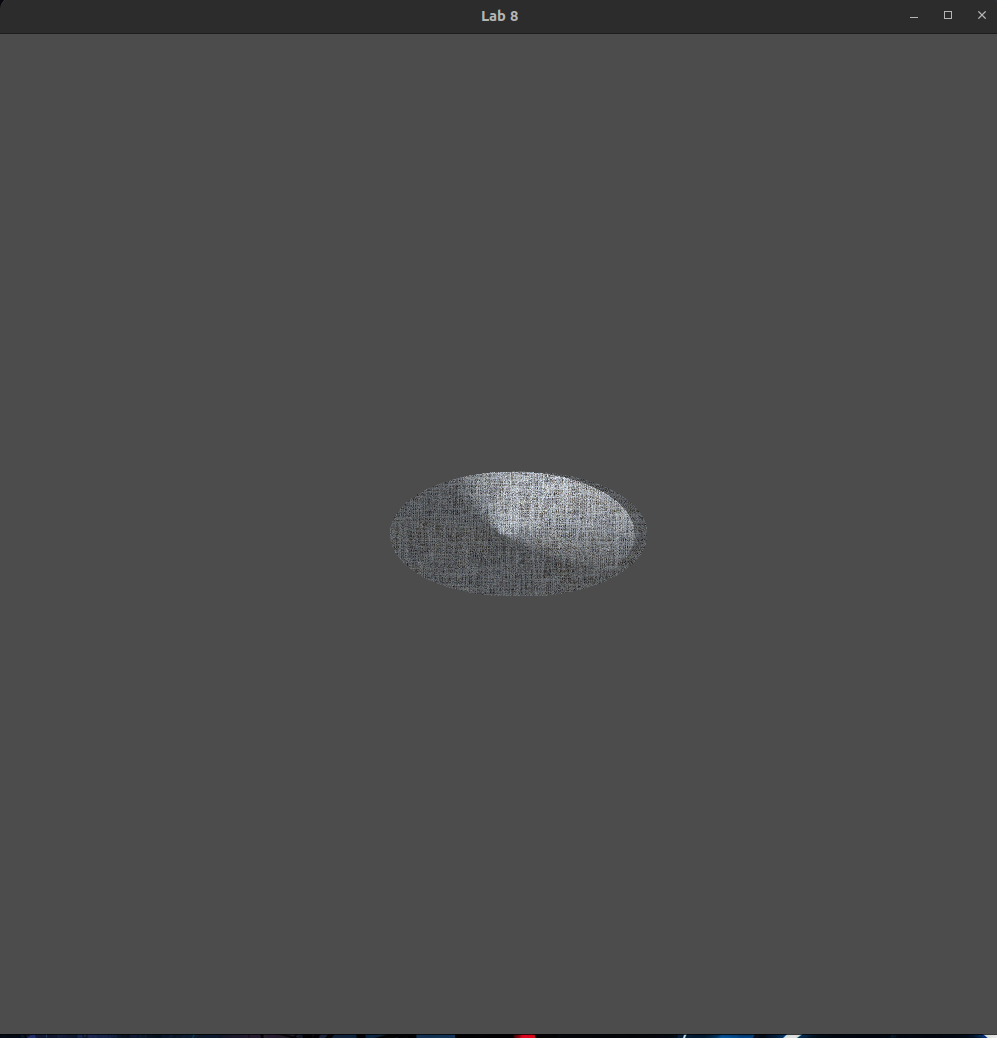
\includegraphics[width=0.8\textwidth]{picture_1.png}
\caption{Без воздействия}
\label{fig:picture_1.png}
\end{figure}

\begin{figure}[!htb]
	\centering
	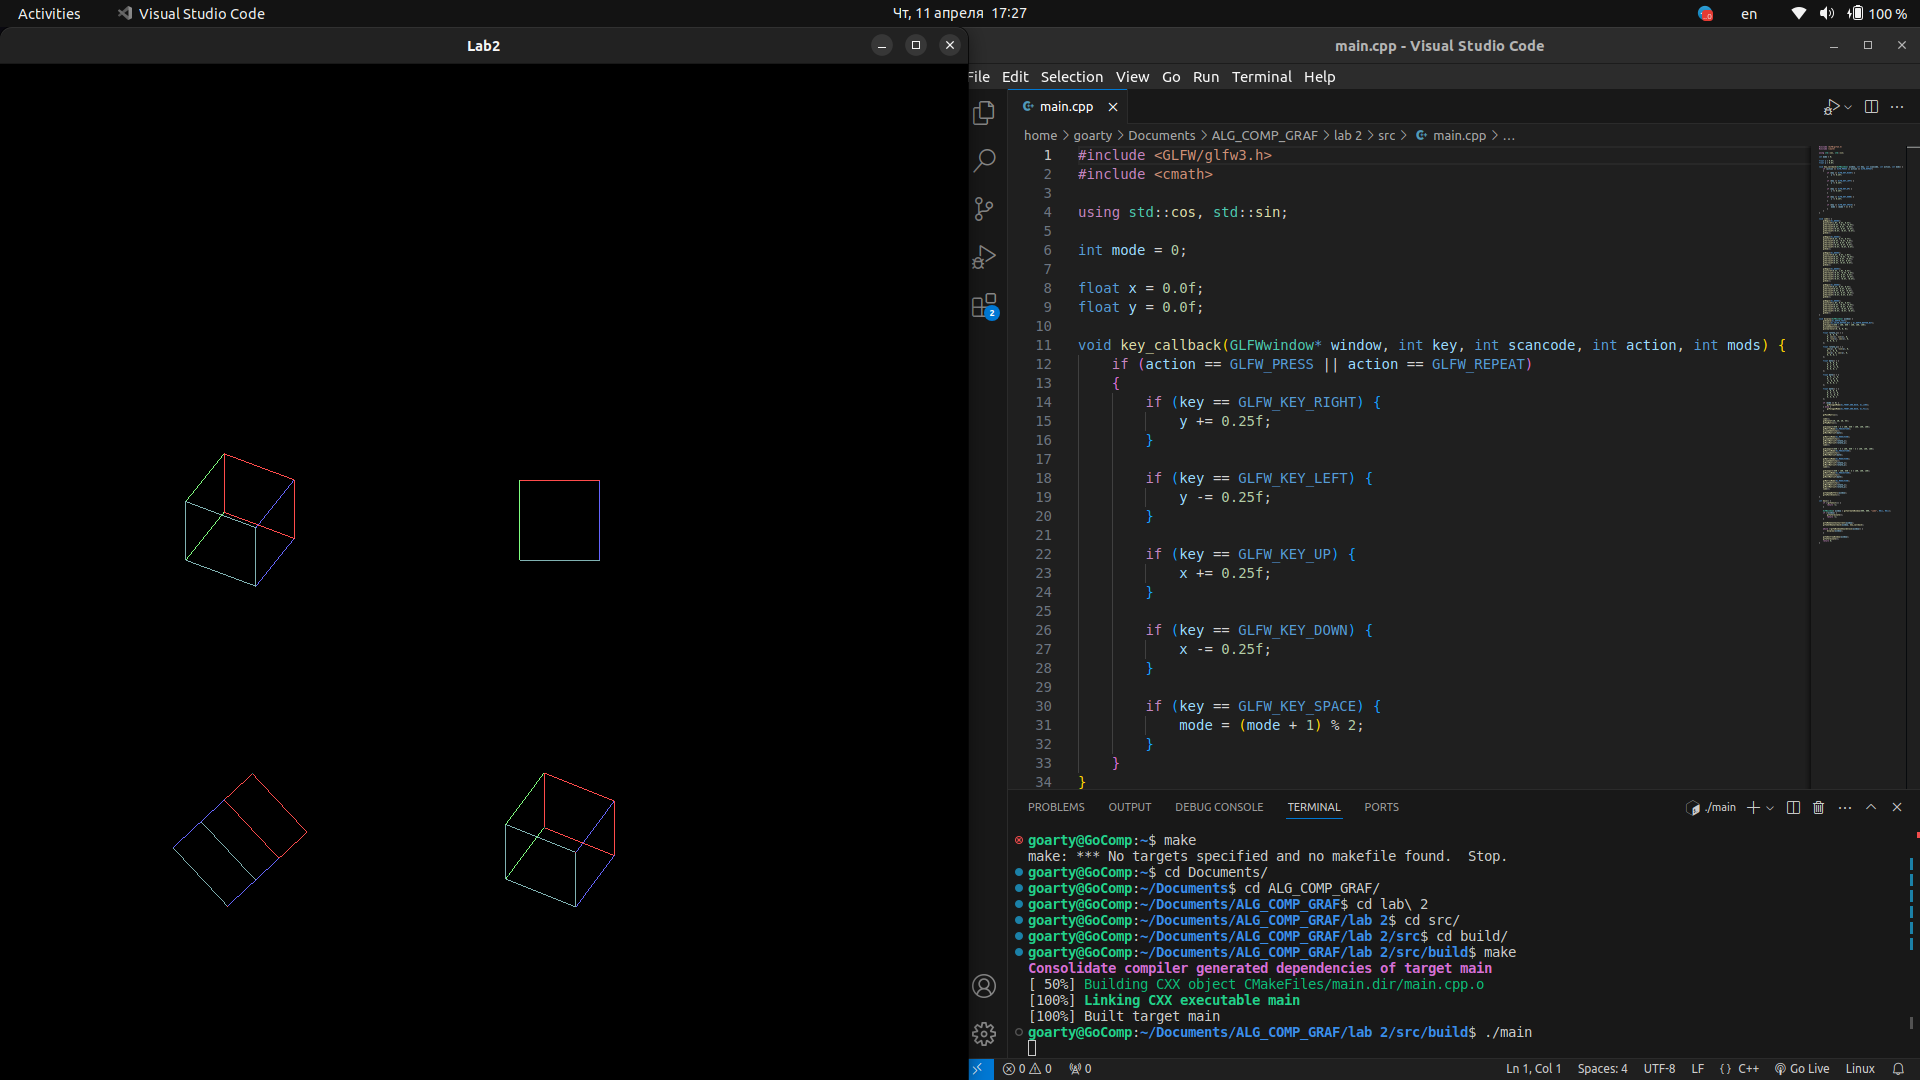
\includegraphics[width=0.8\textwidth]{picture_2.png}
\caption{Повёрнутый}
\label{fig:picture_2.png}
\end{figure}

\begin{figure}[!htb]
	\centering
	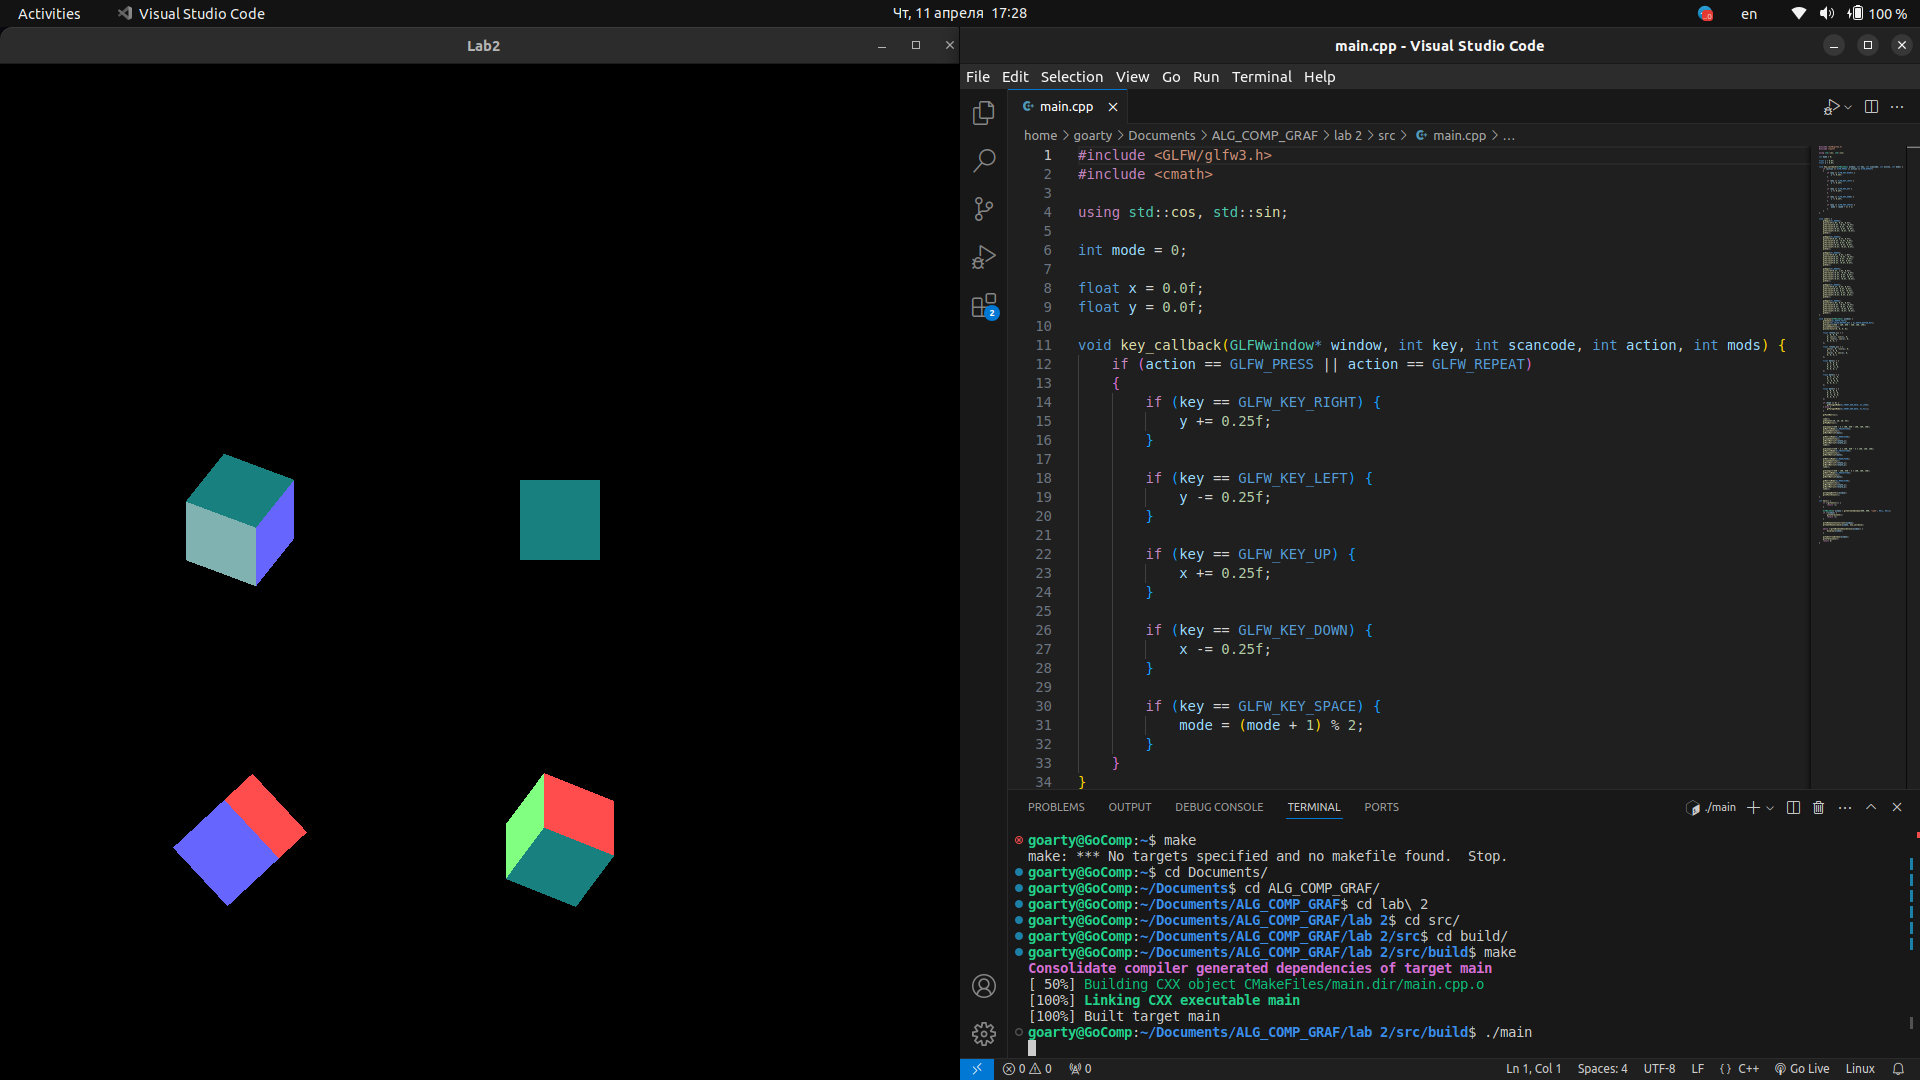
\includegraphics[width=0.8\textwidth]{picture_3.png}
\caption{заполненый}
\label{fig:picture_3.png}
\end{figure}



\end{document}

